\subsection{Modelo OSI}

El modelo OSI es un modelo que abstrae en 7 capas los protocolos involucrados en la comunicación entre dos nodos en una red.

\begin{center}
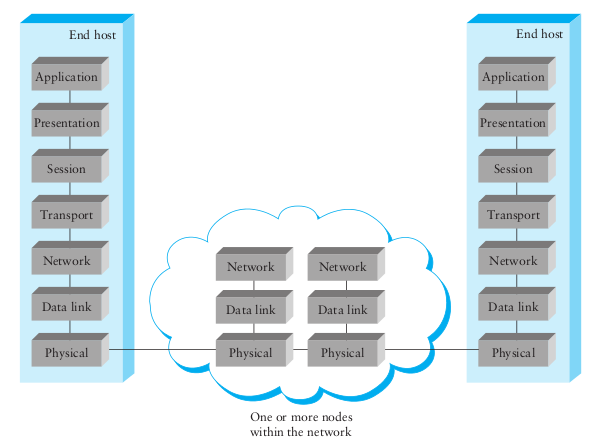
\includegraphics[width=\textwidth/2]{imgs/osi.png}
\end{center}

\subsection{Paquetes IP}

Los paquetes IP\footnote{RFC 791 (IP): https://tools.ietf.org/html/rfc791} son el método principal de intercambio de mensajes entre nodos a nivel de red. Es decir, cuando los nodos pertenecen a distintas redes locales y no tienen acceso la dirección física del otro. El protocolo IP es \textit{best-effort}, por lo tanto existe la posibilidad de que un mensaje nunca llegue a destino. Es más, los routers que implementan RED\footnote{RFC 2309 (RED): https://tools.ietf.org/html/rfc2309}, están configurados para descartar paquetes periódicamente con alguna probabilidad, incluso antes de entrar en un estado de congestión.

\subsection{Paquetes ICMP}

Los paquetes ICMP\footnote{RFC 792 (ICMP): https://tools.ietf.org/html/rfc792} son paquetes de control que no contienen datos, utilizados por los routers para reportar errores en el intercambio de mensajes de una conexión.

\subsection{Traceroute}

Traceroute es una herramienta que permite mostrar la ruta de una conexión entre dos nodos, identificando todos los nodos intermedios y sus respectivos tiempos de demora. Existen distintas implementaciones de Traceroute a diferentes niveles, que brindan ventajas o desventajas en función de ello. Todas se basan en enviar mensajes con el campo TTL (time to live) incrementándose de uno en uno de forma que, los paquetes sean rechazados por los sucesivos routers en la ruta, al haber finalizado su tiempo de vida. El emisor recoge esas respuestas de los routers y genera el camino virtual correspondiente a partir de las ips de los emisores de estos mensajes. Notar que en el caso de los protocolos IP o UDP, donde no se establece una conexión (son orientados a datagramas, no a conexión) es posible que se produzca un cambio de ruta durante el procedimiento. En el momento en que el mensaje llega a destino, se obtiene una respuesta del host objetivo. Esto indica la finalización del Traceroute.
